\documentclass[aspectratio=169]{beamer}              % only frames

% for themes, etc.
\mode<presentation>
\usetheme{Madrid} 
\usecolortheme{crane}

%\usepackage{times}  % fonts are up to you
% The usual suspects
\usepackage{multirow, booktabs, dcolumn, color, graphicx} % Tables\usepackage{graphicx}
\usepackage{amsmath,amssymb,amsthm}
% Strikethrough text
\usepackage{soul}
% Adjust box to fit tabulars
\usepackage{adjustbox}
% Embed video
\usepackage{media9}
% For notes
\usepackage{pgfpages}
\setbeameroption{hide notes} % Only slides
%\setbeameroption{show only notes} % Only notes
%\setbeameroption{show notes on second screen=right} % Both
% Use colors by name
\usepackage{xcolor}
% EMBEDDING VIDEO IS POSSIBLE WITH PDFPC USE PDF PC to present
\usepackage{multimedia}



% The table highlighting for hypothesis discussion.
\usepackage[beamer,customcolors]{hf-tikz}
\usetikzlibrary{calc}

% To use background images
\newenvironment{colorframe}[2][]{%
\setbeamercolor{background canvas}{bg=#1}
\begin{frame}\color{white}}
{\end{frame}}


% To set the hypothesis highlighting boxes red.
\tikzset{hl/.style={
    set fill color=red!80!black!40,
    set border color=red!80!black,
  },
}

% Set Graphics folder
\graphicspath{{./figures/}}


% these will be used later in the title page
\title{Threatlandscape}
\subtitle{Access: Credentials}
\author{Irfan Kanat}
\institute[CBS]{{Department of Digitization}\\ Copenhagen Business School}
%\date{\today}



\begin{document}

% this prints title, author etc. info from above
\begin{frame}

    \titlepage


    \vfill
    {\tiny \centering This work is licensed under a \href{http://creativecommons.org/licenses/by/4.0/}{Creative Commons Attribution 4.0 International License}.}

\end{frame}

\note{In this presentation we focus on how malicious actors gain access to information assets.}

\begin{frame}
    \frametitle{Big Question}
    
    \large How do they gain access?

\end{frame}

\note{Now that we know who all is out there, let us take a look at how they do what they do.

According to DBIR 2021 report, 85\% of the breaches involved some sort of human involvement. 61\% of the breaches involved credentials.}

\begin{frame}
    \frametitle{All Roads Lead to Information}
    
    \begin{itemize}
        \item Credentials
        \begin{itemize}
            \item Legitimate Credentials
            \item Stolen Credentials
            \item Bruteforce
        \end{itemize}
        \item Vulnerabilities 
        \begin{itemize}
            \item Configuration
            \item Bugs
        \end{itemize}
        \item Human Element
        \begin{itemize}
            \item Social Engineering
            \item Insiders
        \end{itemize}
    \end{itemize}

\end{frame}

\note{There are many ways to access information stored on our computing devices. Too many to cover with any real accuracy. 

We will nevertheless cover the broad outlines of the most common ways of gaining access and ways of making these attacks less likely.}



\begin{frame}
    \frametitle{Credentials}

    \begin{columns}
        \begin{column}{0.5\textwidth}

            \begin{itemize}
                \item Legitimate Credentials
                \item Stolen Credentials
                \item Bruteforce
            \end{itemize}
    
        \end{column}

        \begin{column}{0.5\textwidth}

            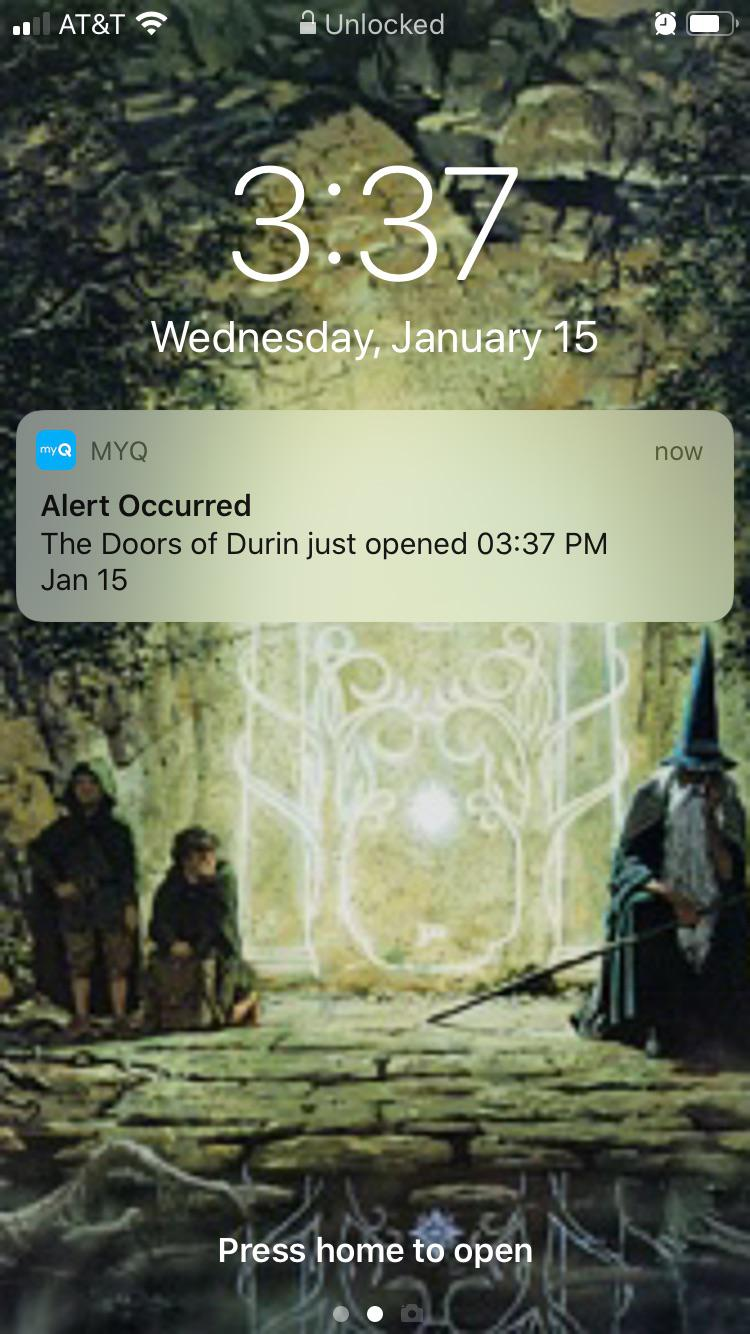
\includegraphics[width = \textwidth, height = .85\textheight, keepaspectratio]{figures/DoorsOfDurin.jpg}

        \end{column}

    \end{columns}
    

\end{frame}

\note{
    Our systems determine who has how much access based on the credentials presented.

    Easiest way to gain access would be to have these credentials. Which is why Phishing attacks are always popular.
}

\begin{frame}
    \frametitle{Insiders and Legitimate Credentials}
    
    \centering
    
    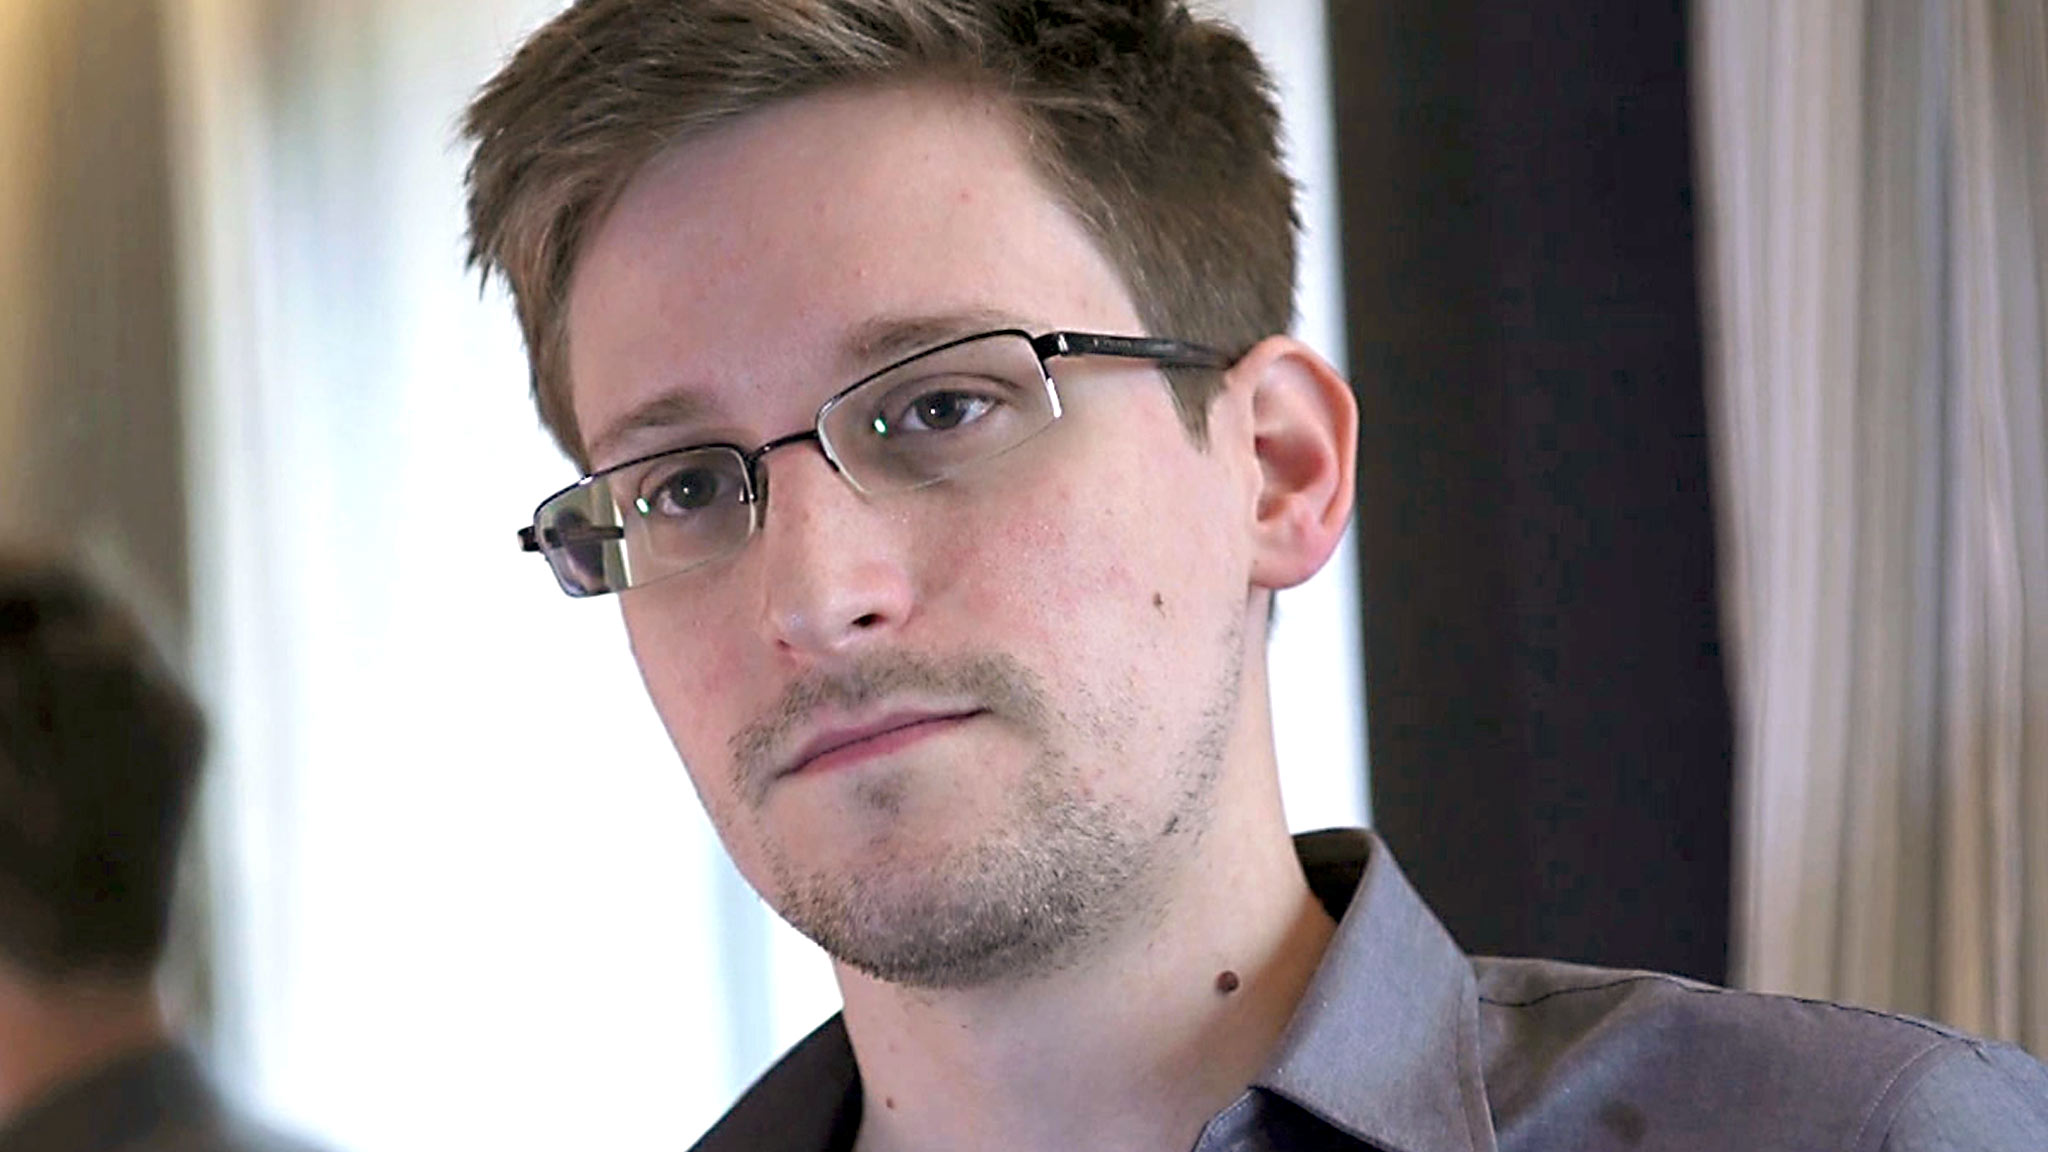
\includegraphics[width = \textwidth, height = .85\textheight, keepaspectratio]{figures/snowden.jpeg}

\end{frame}

\note{
    Organizations need people to carry out their business. This requires a certain level of trust, which is reflected in the access one is granted. 

    We trust that the employee will act with the organizations' best interest in mind with the access they are given. This is part of the employment contract afterall.

    Problems arise when the employees are disgruntled, or conflicts with other interests arise. 

    For example in 2014, a contractor for NSA felt that public interest overrode the interests of the intelligence agency that employed him. He obtained thousands of classfied documents and revealed them to the press. The rest is history.

    No matter what we may think of Edward Snowden and his actions, it is obvious that the process to grant and revoke credentials needs some consideration.
}


\begin{frame}
    \frametitle{Stolen Credentials}
    
    \centering

    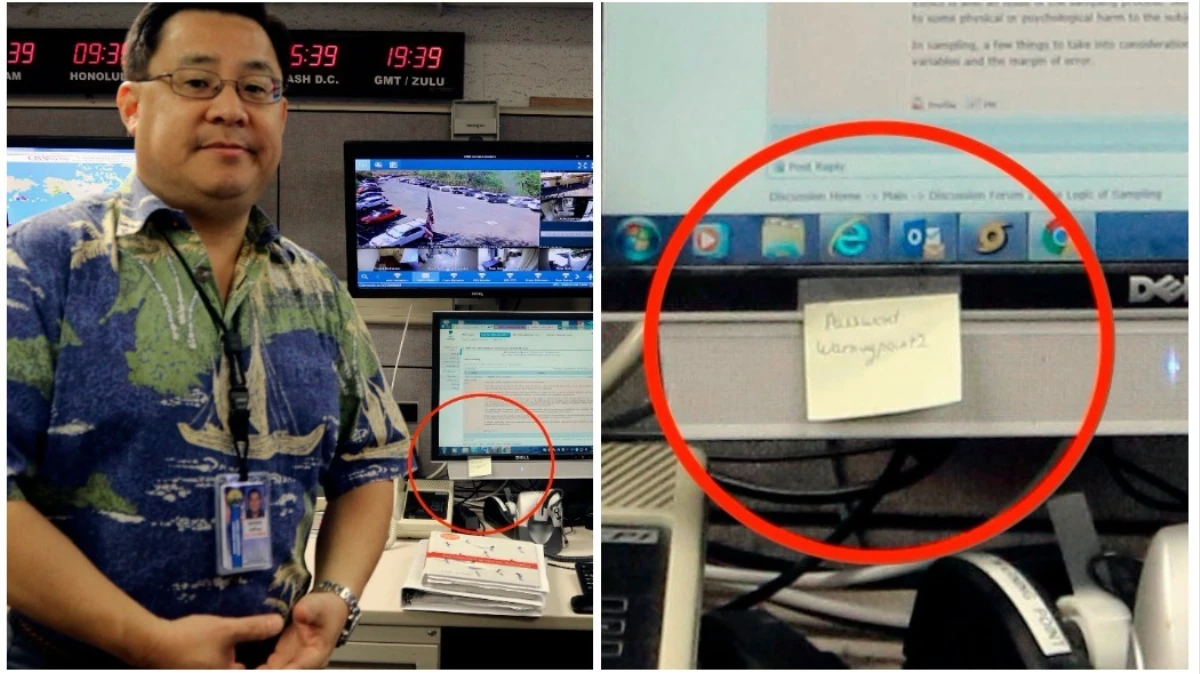
\includegraphics[width = \textwidth, height = .85\textheight, keepaspectratio]{figures/HEMA.png}

\end{frame}

\note{
    When legitimate access is not an option, the next best thing is to borrow the credentials of someone who has access.

    It can be a simple matter of reading what is written on the post-it notes. At this point there have been too many emergency agencies, police stations, and military units embarassed by revealing their passwords on live TV.

    More often though, malicious actors will steal the passwords through phishing or cross site scripting. 

    Phishing is the practice of sending misleading e-mails to legitimate users. The e-mail may include a malware infected file, or a link to a phishing website. Very often when the user clicks the link they are redirected to a legitimate looking website, if they enter their password in this website the password will be passed onto the malicious actors. Similarly, the malware downloaded from phishing e-mails can establish backdoors on users' systems, or steal passwords stored on the system.
}

\begin{frame}
    \frametitle{Brute Force}
    
    \centering

    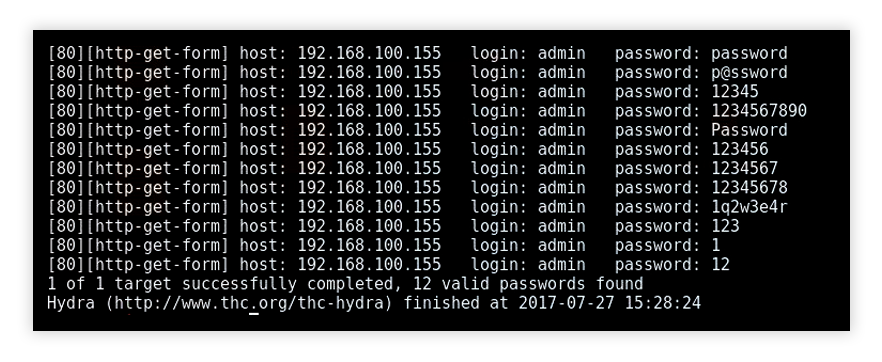
\includegraphics[width = \textwidth, height = .85\textheight, keepaspectratio]{figures/hydra-brute-force-attack.png}

\end{frame}

\note{Brute forcing a password is to throw computational power at the problem. You would try possible passwords until you find one that works.

Most systems that have remote access would have some mechanisms to make brute forcing a password difficult. System may time out or disable user account after certain number of tries for example.

Still, there are ways of brute forcing passwords such as password spraying, attacking a vulnerable protocol (SMB v1 and v2 are notorious), or brute forcing the passwords offline on stolen shadow files for example.}

\begin{frame}
    \frametitle{Some Ways to Keep Credentials Safe}
    
    Don't save your passwords in clear text. \vspace{1em}

    Don't reuse the same password in multiple sites. \vspace{1em}

    Use long and complex passwords. \vspace{1em}

    Use a password manager. \vspace{1em}

    Use multi-factor authentication.

\end{frame}

\note{The proper action depends on the context. Correct control for a bank will not be the same as the corner pizzeria, which will not be the same for a high-school student. Generally though, these tips apply to almost everyone.

To make it harder to steal your credentials, don't store your passwords in clear text. Don't write them down on paper...

Sometimes a website will get hacked and the passwords for the users will be leaked. Then malicious actors may use the same password for the users' accounts on other web sites. You wouldn't want the bad guys to gain access to your bank account because some fan-fiction forum you subscribed to got hacked. So don't reuse the passwords across multiple sites.

To prevent brute forcing your passwords, use long and complex passwords that are a combination of lower, upper case letters, numbers, and symbols. You have these complex passwords that are hard to remember, and you also use a different one for each web site... This is getting hard to remember...

So use a password manager with a really good master-password to keep all those hard to remember passwords safe.

Also use multifactor authentication so that even if your password is stolen, or brute-forced you can still make the attackers job harder. Even if they managed to get through the password, they need to still need to bypass the additional authentication (can be a cell phone app, or a cryptographic key).

For an organization, codifying the above behavior in security policy and system configurations would increase security.
}


\end{document}
